\section{Security Contracts approach}
\label{sec:security-contracts-approach}

We devote this section to the description of our \emph{Security Contracts} approach, which builds on our preliminary work in~\cite{guerin:hal-03217126}. As mentioned above, \emph{Security Contracts} is an extension of the DbC method specially tailored to the representation and monitoring of cyber security patterns. Concretely, we extend DbC so that the contracting party is composed not only of individual classes and methods, but sets of collaborating classes as we may find in security design patterns. Additionally, our extension includes tool support for the instantiation of security patterns as cross-cutting \emph{aspects} on host applications, tool support for the run-time monitoring (and enforcement) of pattern properties (i.e., EuC) and a library of re-usable security patterns. In particular, this section (i) formally describes cyber-security contracts, (ii) presents the application of such contracts to security patterns, and (iii) presents tool support and develops the case of the authenticator pattern to illustrate our approach.

\subsection{Security Contract}

%\begin{equation}
%SecurityContract = SecurityPattern + DbC
%\end{equation}


\begin{figure}
    \centering
%    \includegraphics[width=1.0\columnwidth]    
    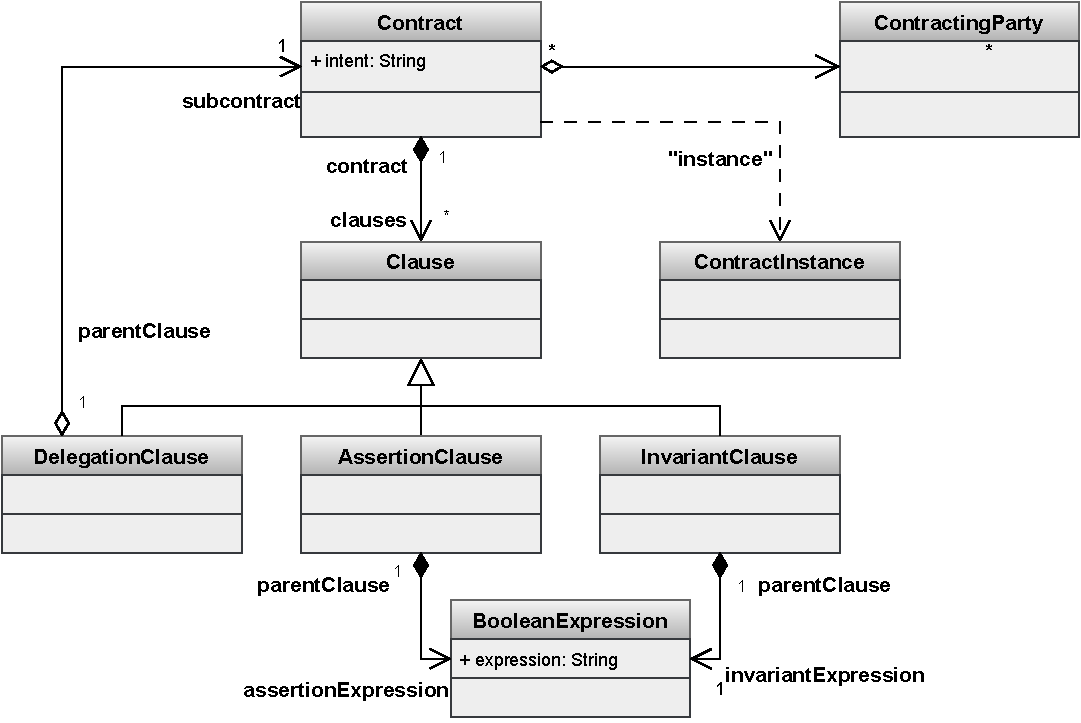
\includegraphics[width=1.0\columnwidth]{figures/MetamodelSecurityContractV3.pdf}
    \caption{Security Contract Metamodel}
    \label{fig:securitycontractmetamodel}
 \end{figure}

 The first component of our approach is a mechanism for the specification of security patterns as contracts. We base this mechanism on a \emph{Security Contracts} metamodel which we depict in Figure~\ref{fig:securitycontractmetamodel} (note that this model is implemented as Java annotations as we explain in Section~\ref{subsec:toolsupport}). The core abstraction of our metamodel is the \emph{Contract} concept which associates formal properties with contracting parties and a run-time instance. 

%Concretely, \emph{Contracts} are associated to a number of \emph{Contracting Parties} (which can be classes, methods, instances, modules, etc), contain a number of \emph{Clauses} and are  Instances of contracts are reified (see the $\emph{ContractInstance} concept)  \emph{Clauses} represent classical DbC pre/post conditions and invariants.a
 
Concretely,  the \textit{Contract} concept has an attribute \textit{intent}, is associated with a collection of contracting parties and is composed of \textit{Clauses}. Additionally, \textit{Contracts} are \emph{realized} in a \emph{ContractInstance} so that we can represent patterns as stateful objets and follow their evolution at run-time. The \textit{intent} is a text that describes, in natural language, the purpose of the contract. The contracting parties are represented by the \textit{ContractingParty} concept and they correspond to the programming entities whose behaviors are subject to the \textit{Contract}. These entities can be classes, methods, instances, modules, etc. A \textit{Contract}  (i.e., a cyber contract) in our approach differs from the classic view of contracts proposed by Meyer in his DbC paradigm: DbC contracting parties can only be classes and methods whereas ours are not limited by their nature (instances, set of classes, programming units, etc.).. Furthermore, the *-* cardinality in the relation between the \textit{Contract} and \textit{ContractingParty} concepts enables the definition of a \textit{Contract} involving multiple \textit{ContractingParties}, potentially of different nature. This relation also provides the possibility to define multiple contracts for a given \textit{ContractingParty}. In our cyber contract context, the \textit{ContractingParties} stand for the entities involved in the security pattern definition. 

Every \textit{Contract} contains a set of \emph{Clauses}. There are three types of \textit{Clauses} that can be added to a \textit{Contract}: \textit{AssertionClause}, \textit{InvariantClause} and \textit{DelegateClause}. A property (in our case, a cyber-security pattern property) which represent properties ensured by the contract refers to one of the two first types of clauses. \textit{AssertionClauses} enable the specification of assertions that need to be verified at a certain time. They extend the notions of precondition and postcondition of the DbC approach by including a temporal aspect. Conversely, \textit{InvariantClauses} are assertions that must always be true, and can therefore be expressed with classical logic. The \textit{DelegateClause} is a concept allowing for responsibilities of a contract to be divided into one or several subcontracts. This mechanism is typically used in the object-oriented paradigm to decompose a contract on the pattern classes, or any decomposition unit of the targeted language.

Assertion and invariant \emph{Clauses} contain a \textit{BooleanExpression}. This concept is an abstraction representing any kind of logic property that one could want to enforce using a contract. In a goal to remain independent of the property expression language, the metamodel does not require any precise expression language. Note however that a constraint exists for the logic used in \textit{BooleanExpressions} within \textit{AssertionClauses}. Such logic must support time-based reasoning.

 
%On essaie de décrire l'approche SecurityContract indépendamment de tout langage de programmation (on pourrait le faire en n'importe quoi). Présenter donc les concepts et les aspects méthodologiques liés à ce qu'est un SecurityContract.
%On y trouve pêle-mêle: des aspects structurels (avec des rôles), des aspects comportementaux, et des propriétés à garantir.
%On continue en disant qu'on a choisi de faire nos expérimentations en Java, et qu'on a choisi Pamela.


\subsection{Contract specification example}
\label{subsection:secureapplication}

%The implementation of the \textit{Authenticator} pattern on the secured application is relatively transparent to the application developer, from a functional point of view. However, the run-time weaving mechanism now explicitly manages %instances of the \textit{Authenticator} pattern (\textit{AuthenticatorPatternInstance}), with their own life cycle that evolves as sessions are created and deleted in the web application. The \textit{SessionInfo} class is now equipped with an %authentication mode, insofar as the methods annotated with \textit{@RequiresAuthentication} (e.g. method \texttt{checkSecure()}, line 50 of the listing \ref{listing:SessionInfo}) can only be executed if the current instance is declared as the %subject of an instance of the \textit{Authenticator} pattern for which authentication has been satisfied. This allows to protect any unauthorized and malicious code call in the context of a vulnerability that would give access to the %execution of this code.a

Let’s exemplify the definition of a security contract for the Authenticator pattern. To do so, we will first use formal boolean expressions in order to describe the contract properties. Note that these boolean expressions suppose the existence of a object oriented representation of the pattern as depicted in Figure~\ref{fig:authclasses} (e.g., we suppose the existence of Classes representing the concepts of the authenticator pattern such as \emph{Subject}). The \textit{Authenticator} pattern intrinsically defines six security properties (four implicit properties and two functional properties), which have been previously introduced as pattern forces in Section~\ref{sec:preliminaries}: 

\begin{enumerate}
    \item \textbf{Unicity of the couple subject/authentication information}
    \begin{equation*}
        P1: \forall a, b \in I_{Subject}, a \ne b \implies a.authInfo \ne b.authInfo
    \end{equation*}
    
    \item \textbf{Authentication information integrity }
    \begin{equation*}
        P2: \forall a \in I_{Subject}, a.authInfo = a.authInfo_{ini}
    \end{equation*}
    
    \item \textbf{Authenticate authority integrity}
    \begin{equation*}
        P3: \forall a \in I_{Subject}, a.authenticator = a.authenticator_{ini}
    \end{equation*}

    \item \textbf{Verification of the validity or an undefined proof of identity}
    \begin{equation*}
      \begin{split}
        &P4: \forall a \in I_{Subject}, (a.idProof = \emptyset) \lor \\&(a.idProof = a.authenticator.request(a.authInfo))
      \end{split}
    \end{equation*}

    \item \textbf{Continue verification of the proof of identity}
    \begin{equation*}
        P5: self.idProof = self.authenticator.request(self.authInfo)
    \end{equation*}
\textbf{Remark:}After authentication, the proof of identity must always match the value initially returned by the query method. The joint verification of properties P4 and P5 guarantees the validity of the proof of identity during the entire session.

    \item \textbf{Post-condition for the method\textit{request(authInfo)}}
    \begin{equation*}
        P6: self.check(authInfo) \lor returnValue = \emptyset
    \end{equation*}
 \end{enumerate}


With these properties and the abstract definition of the Authenticator pattern in Figure~\ref{fig:authclasses} we can define our \emph{authenticator} security contract (note that this pattern is extended with an additional property in Section~\ref{sec:case-study}). Figure \ref{fig:cybercontractXML} shows a simplified XML representation of this contract. This representation illustrates an instantiation of our metamodel on the Authenticator cyber contract. The binding with the Authenticator pattern is explicit and we can see the property P1 as an \textit{InvariantClause} defined at the pattern scope. The delegation mechanism provided with the \textit{DelegateClauses} is also illustrated within this example. Some of the previous properties are indeed within the scope of a single method (P5 and P6). They are thus delegated to the relevant classes using a \textit{DelegateClause} (keyword \textit{Subcontract}) and then to the correct methods.

\begin{figure}
    \centering
 \begin{lstlisting}[breaklines=true, language=XML, basicstyle=\ttfamily\footnotesize, mathescape=true]
<Contract>
    <binding "Authenticator_pattern" />  
    <clauses> 
    <InvariantClause P1/>  
    <Subcontract "SubjectContract">
        <binding "Subject" />
        <InvariantClause P2 $\land$ P3 $\land$ P4/>
        <Subcontract "authenticateContract"s>
            <binding "void authenticate()">
            <ensures P5/>
        </Subcontract>
    </Subcontract>
    <Subcontract "AuthenticatorContract">
        <binding "Authenticator"/>
        <Subcontract "requestContract">
            <binding = "ProofOfIdentity request(AuthenticationInformation authInfo)">
            <ensures P6/>
        </Subcontract>
    </Subcontract>
    </clauses>
</Contract>

\end{lstlisting}
\caption{XML representation of the Authenticator pattern contract}
\label{fig:cybercontractXML}
\end{figure}


\subsection{Deployment, Monitoring and Enforcement}

We have described above a metamodel allowing us to describe security patterns as contracts in an abstract manner. For these contracts to have a practical use we need the means to: 1) deploy them in host applications which need to be secured; and 2) monitor then at run-time to both, verify and enforce the contract properties. 

For the operationalization of our \emph{Security Contracts} we choose to follow an Aspect Oriented Approach. Indeed, security mechanisms constitute a classical example of cross-cutting concern and thus, AoP appears as a natural choice. In our approach, abstract \emph{Security Contracts} as defined above are translated to a sort of \emph{advices} which encapsulate the properties to monitor and enforce at run-time. Details of this process are given in Section~\ref{subsec:toolsupport} where we describe a prototype implementation of our approach for the Java ecosystem.


\subsection{Tool Support}
\label{subsec:toolsupport}

In order to demonstrate the feasibility of our approach, a prototype implementation have been developed for the Java ecosystem. It builds on top of the PAMELA framework~\cite{guerin:hal-03217126}. PAMELA is a Java modelling framework which focuses on bridging the gap between software modelling and code implementation. In this context, PAMELA modelling framework proposes an approach where models are directly weaved in source code by means of Java annotations. Thus, it does not require code generation. That way, both model and source-code coexist in the same artifact.

\begin{figure}
    \centering
    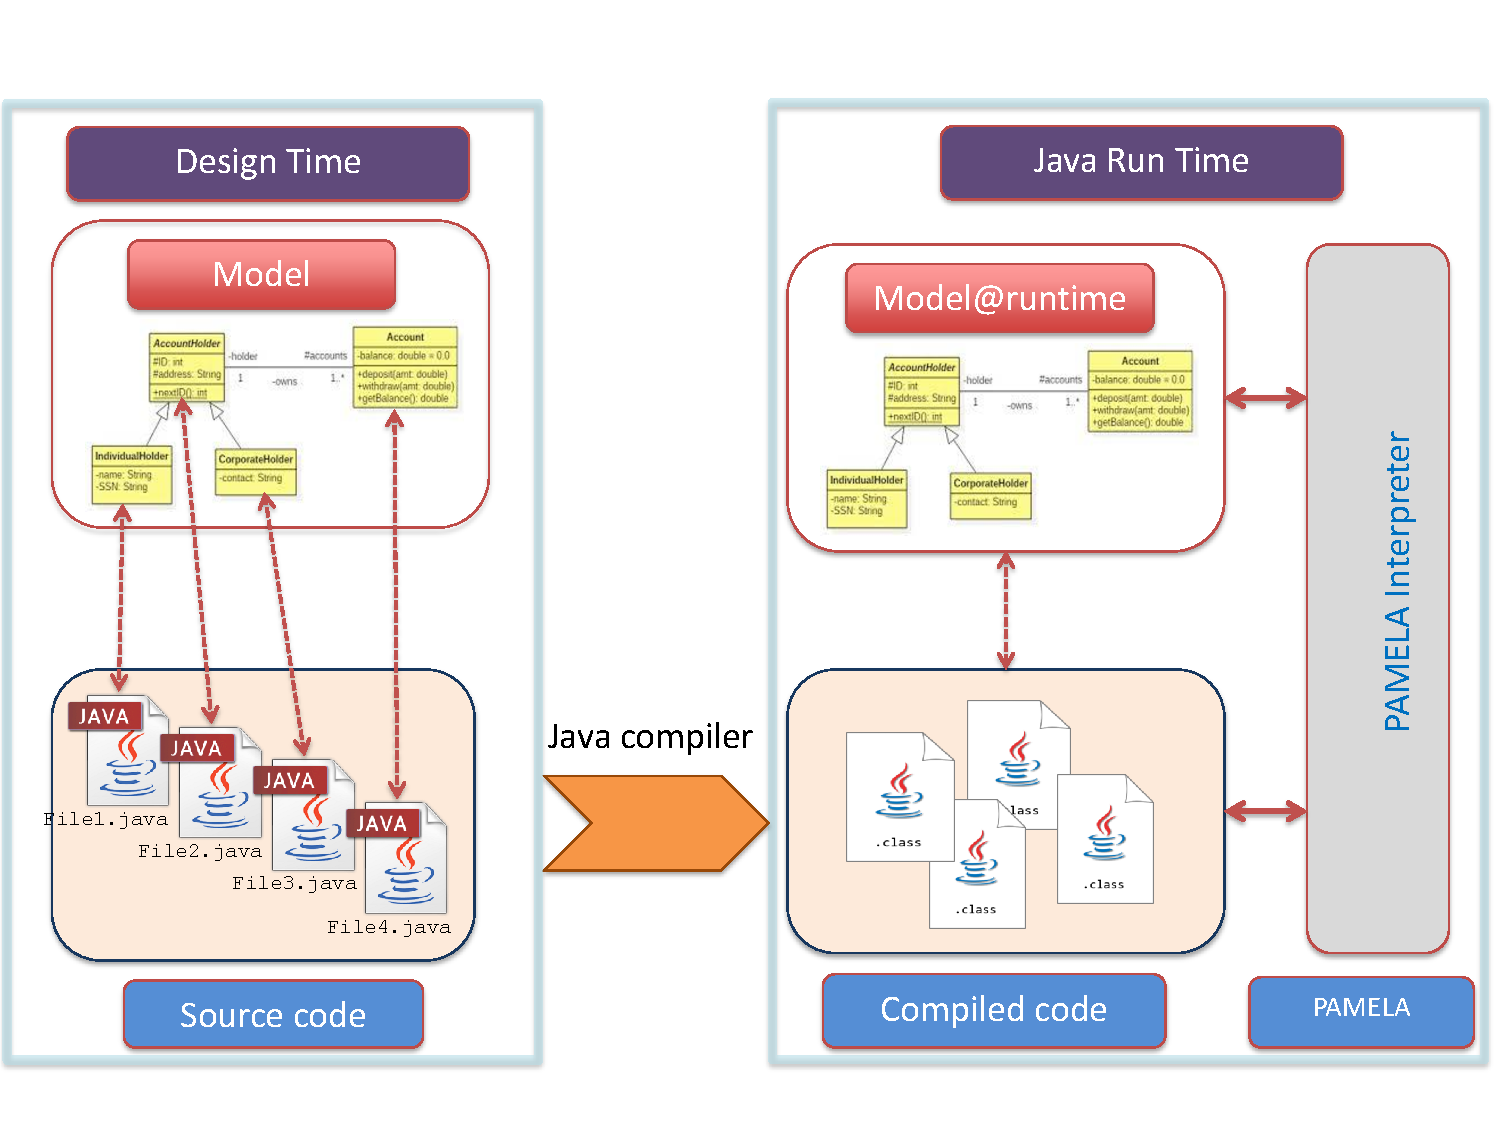
\includegraphics[width=1.0 \columnwidth]{figures/PamelaVisionV2.pdf}
    \caption{Overview of the PAMELA approach}
    \label{fig:PamelaVision}
\end{figure}

Figure \ref{fig:PamelaVision} illustrates the PAMELA framework where we have at design time (left side of the figure) the model weaved in source code files based on the Java annotations and at run-time (right side of the figure) the PAMELA interpreter ensuring the link between the model behavior and the application Java byte-code. Resulting execution is a combination of (i) executing plain Java byte-code as the result of the basic compilation of source code, and (ii) an embedded PAMELA interpreter executing PAMELA model semantics. From an implementation standpoint, PAMELA uses \emph{javassist} reflection library including the \texttt{MethodHandler} mechanism. Based on this support, the Java dynamic binding is overridden to provide the call of the PAMELA model behavior when an object method is invoked. 

In our current scenario, \emph{security contracts} become PAMELA models to be weaved in host applications. We need however to extend the PAMELA framework to include our notion of \emph{Pattern}, i.e. a composition of multiple classes, known as \emph{Stakeholders}, whose expected behavior is defined in a pattern contract, along with formal properties which must be ensured at run-time. More specifically, implementing \emph{Patterns} with PAMELA provides:
\begin{itemize}
    \item the ability to monitor the execution of the code;
    \item the ability to offer extra structural and behavioral features, executed by the PAMELA interpreter;
    \item a representation of \emph{Patterns} as stateful objects. Such objects can then evolve throughout run-time and compute assertions using any paradigms (e.g., LTL - Linear Temporal Logic);
    \item the ability of having multiple extension points. In other words, the ability to create new patterns, or to redefine or specialize existing ones.
\end{itemize}

\emph{Patterns} are defined in PAMELA using three classes, each one representing a different conceptual level:
\begin{itemize}
    \item a \mytexttt{PatternFactory}. This class is responsible for identifying, at run-time, the declared patterns in the Java byte-code.
    \item a \mytexttt{PatternDefinition}. This class represents an occurrence of the pattern in the supplied byte-code. It has the responsibility of maintaining links with all classes and methods involved in the pattern, as well as managing the life-cycle of its \mytexttt{PatternInstances}.
    \item a \mytexttt{PatternInstance}. This class represents the instance of a pattern at run-time. It is responsible for maintaining the pattern state and providing pattern behavior and contract enforcement.
\end{itemize}

To declare a \emph{Pattern} on existing code, pattern elements such as \emph{Pattern Stakeholders} and methods need to be annotated with provided pattern-specific  annotations. These annotations will be discovered at run-time by the \mytexttt{PatternFactory} and stored in \mytexttt{PatternDefinition} attributes.



\subsubsection{The \textit{Authenticator} Security Contract in PAMELA}
\label{subsec:AuthenticatorSecurityContract}

In order to illustrate the main features of our prototype, we present here how our running example, i.e., the \emph{Authenticator} pattern is implemented with PAMELA and its extension for security contracts. In that sense, Figure~\ref{fig:PAMELAAuthenticatorCD} presents the PAMELA class structure for security contracts instantiated for the  Authenticator pattern. Note that each attribute of the \mytexttt{AuthenticatorPatternDefinition} class has a corresponding annotation (displayed as a comment). Then, the code excerpt in Figure~\ref{fig:ExampleOfAuthenticatorPattern} shows how the Authenticator pattern is used by means of annotations to an existing base of code in which an instance of the \texttt{Manager} class plays the \emph{Authenticator} role, while an instance of the \texttt{Client} class plays the \emph{Subject} role. At run-time, both functional code and security pattern logic, i.e pattern behavior and contract enforcement, are weaved by the PAMELA framework. 
More specifically, \mytexttt{PatternDefinition} classes implement the \mytexttt{isMethodInvolvedInPattern} which returns \mytexttt{true} for all methods which need to be handled by the associated \mytexttt{PatternInstances}. This allows, for instance, for the pattern contract properties to be checked at run-time before and/or after any method of interest. In the case of the Authenticator pattern, the \texttt{AuthenticatorPatternInstance} objects will check the invariants of the pattern contract before and after every call to \emph{Subject} and \emph{Authenticator} classes. These checks are performed by the \texttt{checkInvariant} method. These mappings are summarised in Figure~\ref{fig:AuthenticatorPattern}. 

\begin{figure}
    \centering
    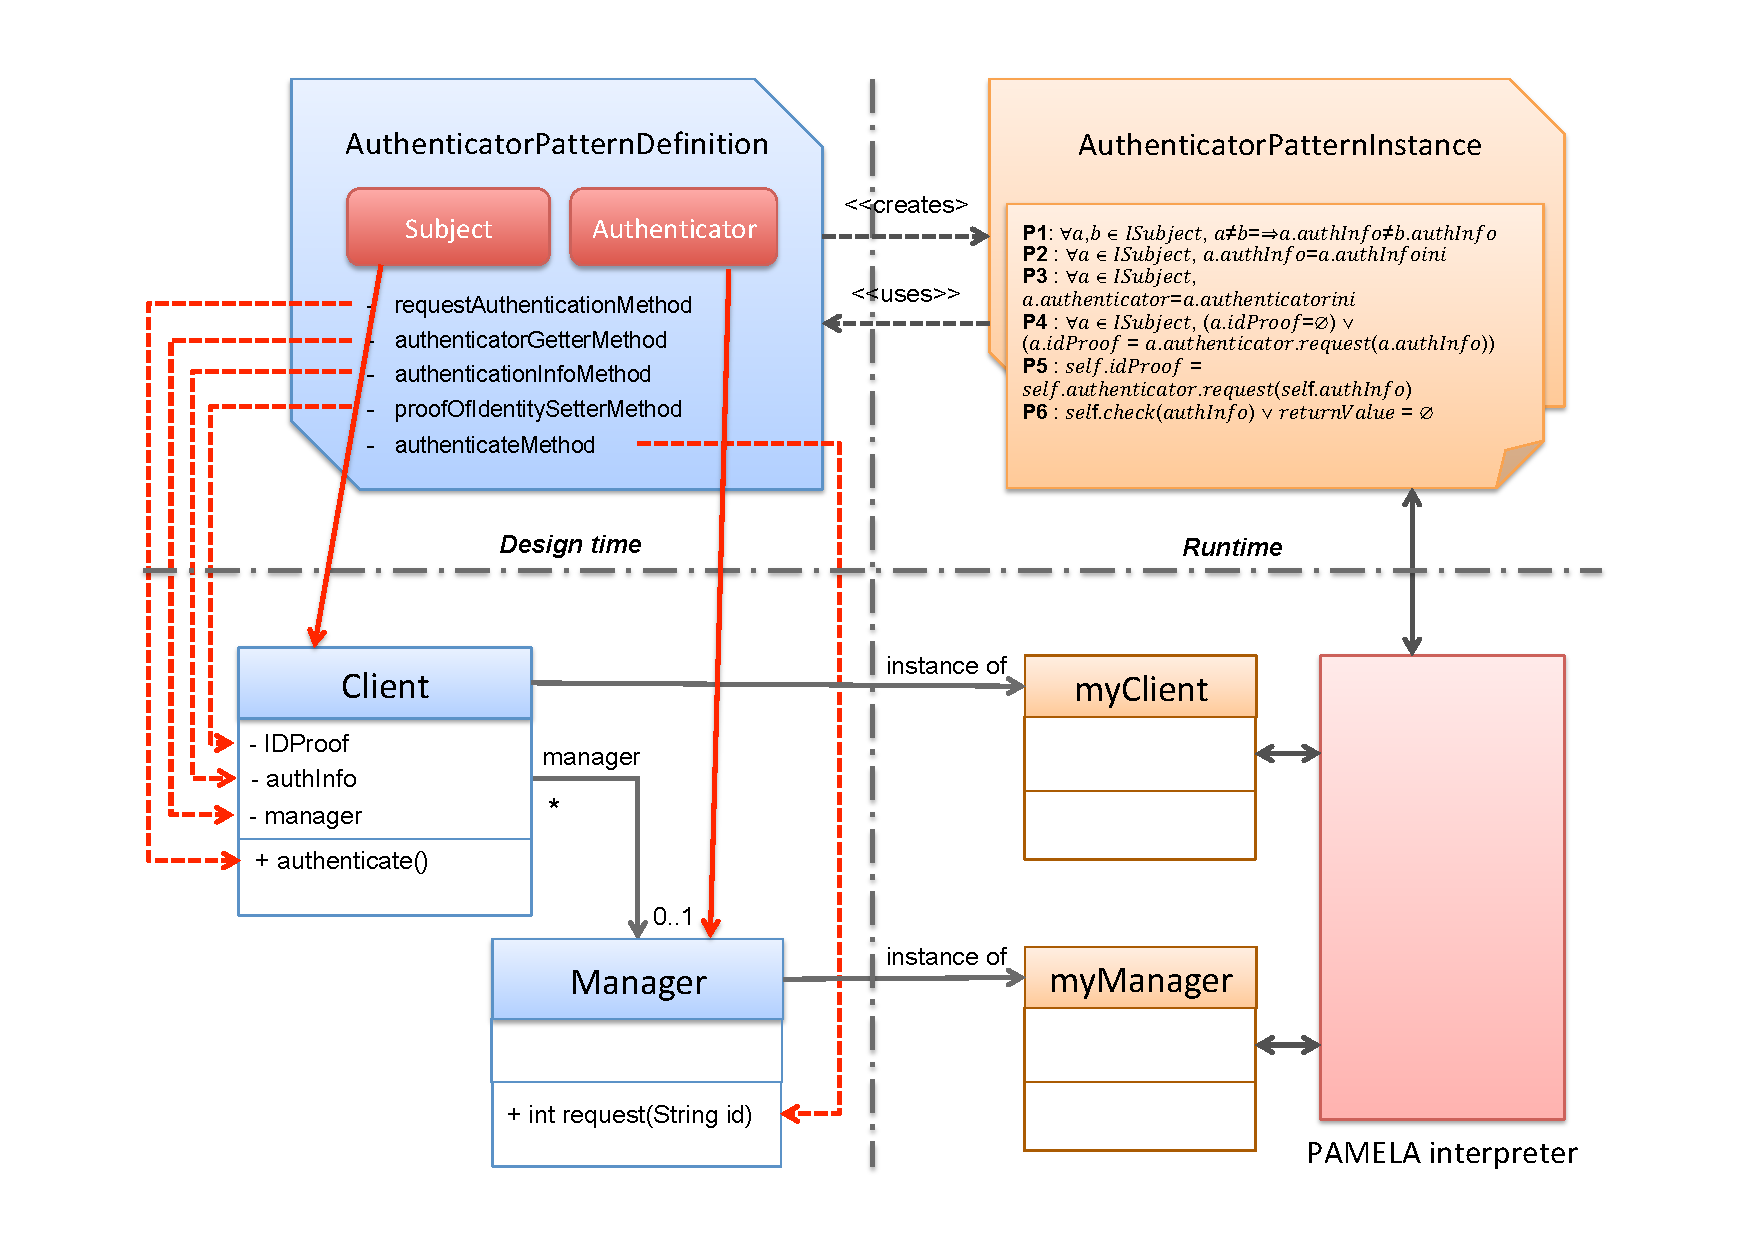
\includegraphics[width=1.0 \columnwidth]{figures/AuthenticatorPattern4.pdf}
    \caption{PAMELA vision of the authenticator pattern}
    \label{fig:AuthenticatorPattern}
\end{figure}

Note that the user only needs to annotate his code and PAMELA will automatically handle the pattern business logic (both, pattern behavior and assertion checking). For more details about this example we direct the reader to our previous publication~\cite{silva2020contract}.

\begin{comment}
\begin{figure}
    \centering
    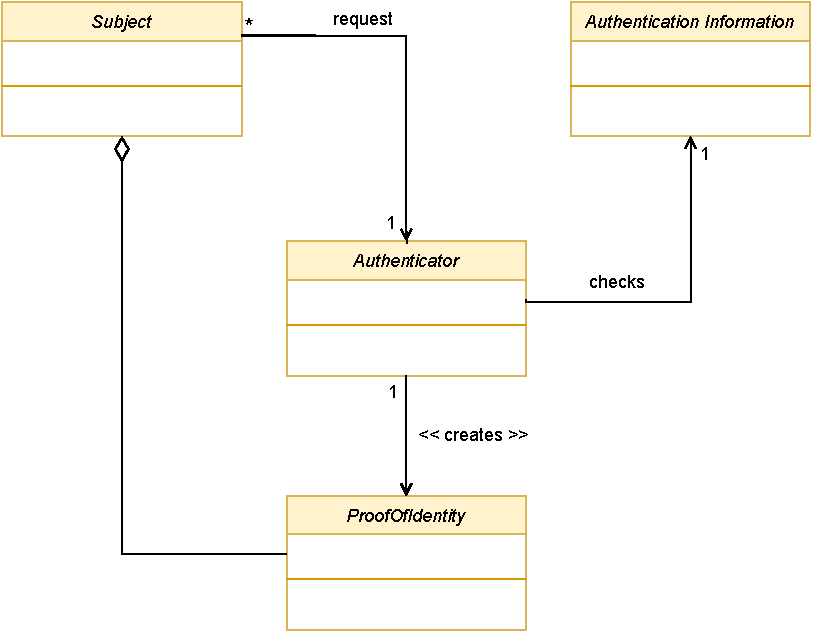
\includegraphics[width=1.0\columnwidth]{figures/AuthenticationClassDiagram.pdf}
    \caption{UML class diagram of the Authenticator security contract}
    \label{fig:authenticatorClassDiagram}
 \end{figure}
\end{comment}

\begin{figure}
    \centering
    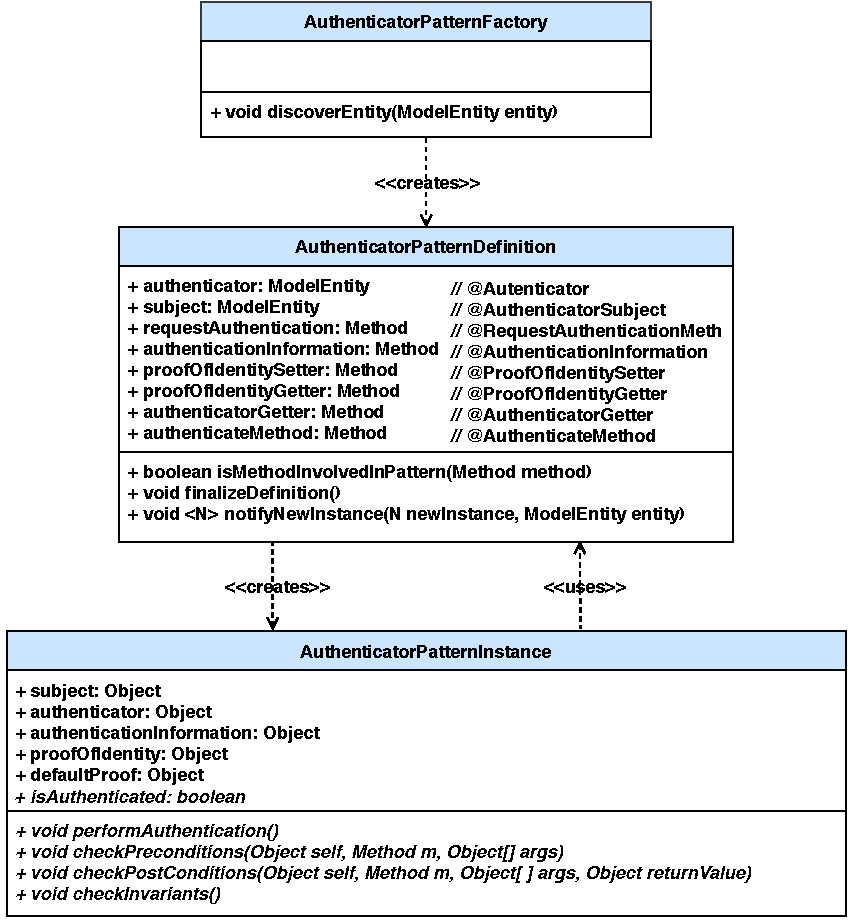
\includegraphics[width=0.8 \columnwidth]{figures/PAMELAAuthenticator_CD.pdf}
    \caption{PAMELA Authenticator pattern class diagram.}
    \label{fig:PAMELAAuthenticatorCD}
\end{figure}

\begin{comment}
    
\begin{figure}
    \centering
    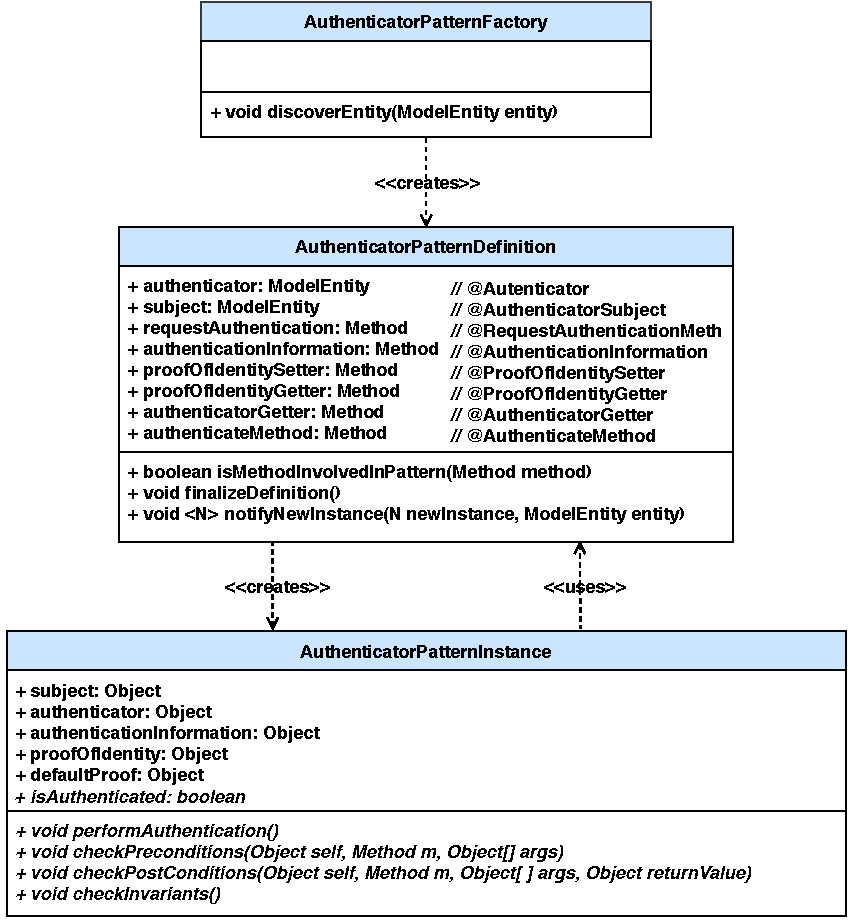
\includegraphics[width=1.0 \columnwidth]{figures/PAMELAAuthenticator_CD.pdf}
    \caption{PAMELA vision of the authenticator pattern}
    \label{fig:AuthenticatorPattern}
\end{figure}
\end{comment}




\begin{figure}
    \centering
\begin{lstlisting}[language=Java,basicstyle=\ttfamily\footnotesize]
@ModelEntity 
@Authenticator(patternID = "PatternId")
public class Manager {

	@RequestAuthentication(patternID = "PatternId")
	public int request(@AuthenticationInformation(
        patternID = "PatternId", paramID = "id") String id) {
		return ...;
	}
}

@ModelEntity
@AuthenticatorSubject(patternID = "PatternId")
public class Client {

	public Client(Manager authenticator, String id) {
		...
	}

	@AuthenticationInformation(patternID = "PatternId", paramID = "id")
	public String getAuthInfo() {
		return ...;
	}

	@ProofOfIdentityGetter(patternID = "PatternId")
	public int getIDProof() {
		return ...;
	}

	@AuthenticatorGetter(patternID = "PatternId")
	public Manager getManager() {
		return ...;
	}

	@AuthenticateMethod(patternID = "PatternId")
	public void authenticate() {
		setIDProof(getManager().request(getAuthInfo()));
	}

	@RequiresAuthentication
	public void securedMethod() {
		...
	}
}
\end{lstlisting}
    \caption{Example showing how to use the \textit{Authenticator} defined as a PAMELA security contract}
    \label{fig:ExampleOfAuthenticatorPattern}
\end{figure}


%\begin{figure}
%    \centering
%    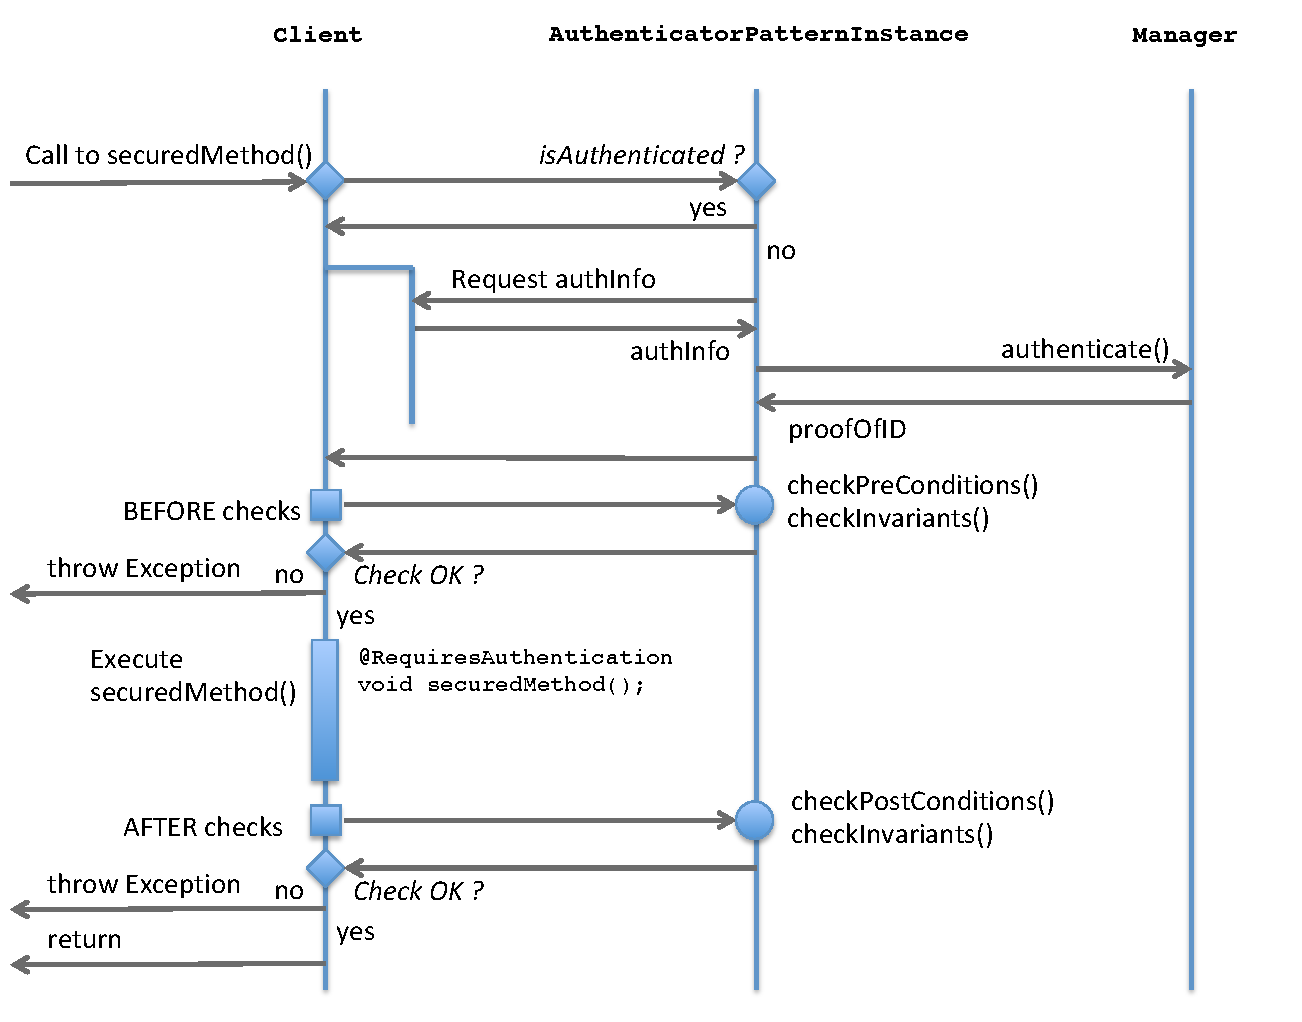
\includegraphics[width=1.0 \columnwidth]{figures/AuthenticatorControlFlow.pdf}
%    \caption{Authenticator control flow}
%    \label{fig:AuthenticatorControlFlow}
%\end{figure}


\subsubsection{Security Contracts Library}

One of the strengths our approach is the separation between the definition of the abstract pattern and their deployment on a host application, as this permits the re-use of well tested and verified patterns. In this sense, our tool support includes a library of off-the-shelf patterns ready to be deployed by application developers in their source code. As of now this library includes the following patterns:

\begin{itemize}
    \item Authenticator
    \item Authorization
    \item Single access point
    \item Owner
    \item Role-based access control
\end{itemize}

Details about this patterns, their features and how to use them are available in the project's web site\footnote{https://www.openflexo.org/pamela/docs/category/security-features/}. More patterns will be added in the near future as we continue developing our framework.

